
\documentclass[oneside,a4paper]{book}
%\pagestyle{headings}


%=============================================================================

\usepackage{amsthm}
\usepackage{xspace}
\usepackage{float}
\usepackage{ifthen}
\usepackage{amsbsy}
\usepackage{amssymb}
\usepackage{balance}
\usepackage{booktabs}
\usepackage{array, graphicx}
\usepackage{rotating}
\usepackage{multirow}
\usepackage{needspace}
\usepackage{microtype}
\usepackage{bold-extra}
\usepackage{geometry}
\usepackage{varioref}
\usepackage[dvipsnames]{xcolor, subcaption}
\usepackage{textcomp}
\usepackage{listings}
\usepackage[normalem]{ulem} %emphasize still italic
\usepackage{ucs}

% \usepackage[utf8]{inputenc}
% \usepackage[htt]{hyphenat}
\usepackage{times}
\usepackage{url}
\usepackage{alltt}
\usepackage{amsmath}
\usepackage{xfrac}
\usepackage{subfigure}
\usepackage{appendix}
\usepackage{stmaryrd}   % for the \shortuparrow
\usepackage[utopia]{quotchap}
\usepackage{tikz}
\usetikzlibrary{snakes}
\tikzset{>=latex}

\usepackage{setspace}
\usepackage[numbers, sort&compress]{natbib}
\usepackage{mdwlist}        % support for better spaced lists
% allows for temporary adjustment of side margins
\usepackage{chngpage}
\usepackage[normalem]{ulem}


% constants

\newcounter{qcounter}

% commands
\newcommand{\n}{$\cdot$}
\newcommand{\y}{\checkmark}
\newcommand{\subscript}[1]{$_{\textrm{\footnotesize{#1}}}$}
\newcommand{\superscript}[1]{$^{\textrm{\footnotesize{#1}}}$}
\newcommand{\vertical}[1]{\raisebox{-4em}{\begin{sideways}{#1}\end{sideways}}}

\newboolean{showedits}
\setboolean{showedits}{true} % toggle to show or hide edits
\ifthenelse{\boolean{showedits}}
{
       \newcommand{\ugh}[1]{\textcolor{red}{\uwave{#1}}} % please rephrase
       \newcommand{\ins}[1]{\textcolor{blue}{\uline{#1}}} % please insert
       \newcommand{\del}[1]{\textcolor{red}{\sout{#1}}} % please delete
       \newcommand{\chg}[2]{\textcolor{red}{\sout{#1}}{\ra}\textcolor{blue}{\uline{#2}}} % please change
}{
       \newcommand{\ugh}[1]{#1} % please rephrase
       \newcommand{\ins}[1]{#1} % please insert
       \newcommand{\del}[1]{} % please delete
       \newcommand{\chg}[2]{#2}
}


% ============================================================================
% Put edit comments in a really ugly standout display

\usepackage{xcolor}
\usepackage[normalem]{ulem}
\newcommand{\ra}{$\rightarrow$}


% comments \nb{label}{color}{text}
\newboolean{showcomments}
\setboolean{showcomments}{true}
\ifthenelse{\boolean{showcomments}}
    {\newcommand{\nb}[3]{
        {\colorbox{#2}{\bfseries\sffamily\scriptsize\textcolor{white}{#1}}}
        {\textcolor{#2}{\sf\small$\blacktriangleright$\textit{#3}$\blacktriangleleft$}}}
     \newcommand{\version}{\emph{\scriptsize$-$Id$-$}}
%	 \newcommand{\ugh}[1]{\textcolor{red}{\uwave{#1}}} % please rephrase
%	 \newcommand{\ins}[1]{\textcolor{blue}{\uline{#1}}} % please insert
%	 \newcommand{\del}[1]{\textcolor{red}{\sout{#1}}} % please delete
%	 \newcommand{\chg}[2]{\textcolor{red}{\sout{#1}}{\ra}\textcolor{blue}{\uline{#2}}} % please change
	 \newcommand{\chk}[1]{\textcolor{ForestGreen}{#1}} % changed, please check
	}
    {\newcommand{\nb}[3]{}
     \newcommand{\version}{}
	\newcommand{\chk}[1]{} % changed, please check
	}

% ============================================================================
% Make quotes be italic
\renewenvironment{quote}
    {\list{}{\rightmargin\leftmargin}%
     \item\relax\begin{it}}
    {\end{it}\endlist}

\newcommand{\ttimes}{\ensuremath{\times}}

%=============================================================================

\newcommand{\needlines}[1]{\Needspace{#1\baselineskip}}

% source code
\usepackage{xcolor}
\usepackage{textcomp}
\usepackage{listings}
\definecolor{source}{gray}{0.9}
\lstset{
	language={},
	% characters
	tabsize=3,
	upquote=true,
	escapechar={!},
	keepspaces=true,
	breaklines=false,
	alsoletter={:},
	breakautoindent=true,
	columns=fullflexible,
	showstringspaces=false,
	basicstyle=\footnotesize\ttfamily,
	% background
	frame=single,
    framerule=0pt,
	backgroundcolor=\color{source},
	% numbering
	numbersep=5pt,
	numberstyle=\tiny,
	numberfirstline=true,
	% captioning
	captionpos=b,
	numberbychapter=false,
	% formatting (html)
	moredelim=[is][\textbf]{<b>}{</b>},
	moredelim=[is][\textit]{<i>}{</i>},
	moredelim=[is][\uline]{<u>}{</u>}}
\newcommand{\ct}{\lstinline[backgroundcolor=\color{white},basicstyle=\footnotesize\ttfamily]}
\newcommand{\lct}[1]{{\small\tt #1}}


%----------------------------------------------------------------------------
% references
\newcommand{\tabref}[1]{\hyperref[{tab:#1}]{Table~\ref*{tab:#1}}}
\newcommand{\figref}[1]{\hyperref[{fig:#1}]{Figure~\ref*{fig:#1}}}
\newcommand{\secref}[1]{\hyperref[{sec:#1}]{Section~\ref*{sec:#1}}}
\newcommand{\lstref}[1]{\hyperref[{lst:#1}]{Listing~\ref*{lst:#1}}}
\newcommand{\charef}[1]{\hyperref[{cha:#1}]{Chapter~\ref*{cha:#1}}}
%----------------------------------------------------------------------------

% abbreviations
\tracingcolors 4
\setcounter{tocdepth}{3}
\setcounter{secnumdepth}{3}
\newcommand{\ie}{\emph{i.e.,}\xspace}
\newcommand{\eg}{\emph{e.g.,}\xspace}
\newcommand{\etc}{\emph{etc.}\xspace}
\newcommand{\etal}{\emph{et al.}\xspace}


\newcommand{\newevenside}{
	\ifthenelse{\isodd{\thepage}}{\newpage}{
	\newpage
        \phantom{placeholder} % doesn't appear on page
	\thispagestyle{empty} % if want no header/footer
	\newpage
	}
}

\def\stretchfactor{1}
\newcommand{\mychapter}[1]{\setstretch{1}
    \chapter{#1}\setstretch{\stretchfactor}}

%----------------------------------------------------------------------------
\newcommand{\lessSpace}{\vspace{-1em}}
\DeclareGraphicsExtensions{.pdf,.png}
\graphicspath{{images/}}
\newcommand{\fig}[4]{
	\begin{figure}[#1]
		\centering
		\includegraphics[width=#2\textwidth]{#3}
		\lessSpace
		\caption{\label{fig:#3}#4}
	\end{figure}}

% ===========================================================================


\newcommand{\thesistitle}{Title of the Thesis}
\newcommand{\thesisauthor}{Sophie Gabriela Pfister}
\newcommand{\thesisleiter}{Name of the Supervisor}
\newcommand{\thesisasst}{Name of the Assistant}
\newcommand{\thesissubtitle}{Thesis subtitle}
\newcommand{\thesisdate}{Month 2025}



% ===========================================================================

\usepackage[ colorlinks=true, urlcolor=black, linkcolor=black,
			citecolor=black, bookmarksnumbered=true, bookmarks=true,
			plainpages=false,
			pdftitle={\thesistitle}, pdfauthor={\thesisauthor},
			pdfsubject={\thesissubtitle}, pdfpagelabels]{hyperref}

\newcommand{\hrref}[2]{\hyperref}
% ===========================================================================
% ===========================================================================


% D O C U M E N T
% % % % % % % % % % % % % % % % % % % % % % % % % % % % % % % % % %
\begin{document}

% T I T L E
% % % % % % % % % % % % % % % % % % % % % % % % % % % % % % % % % %
\begin{titlepage}  
  \begin{center}  
  
  \begin{figure}[t]  
  \vspace*{-2cm}        % to move header logo at the top 
  \center{
\includegraphics[scale=0.2]{logos/MSc_quer.png}}
  \vspace{0.4in}     
  \end{figure}

    \thispagestyle{empty}
    
    {\bfseries\Huge \thesistitle \par
    \Large \vspace{0.1in} \thesissubtitle \par}

    \vspace{0.3in} 
    \LARGE{\textbf{Master Thesis} \\}
    \vspace{0.4in}

    {\Large \thesisauthor}
    
    \vspace{0.3in}
%    {\Large University of Bern \par}
    {\Large Philosophisch-naturwissenschaftlichen Fakult\"{a}t \\
            der Universit\"{a}t Bern \par}
    \vfill
    {\Large \thesisdate \par}
  

  \vspace{0.9in}
 
  % === Logos ==============================================     
  \begin{figure}[htp]
    \centering
    
\includegraphics[scale=0.30]{logos/UNI_Bern.png}\hfill
    
\includegraphics[scale=0.30]{logos/UNI_Neuenburg.png}\hfill
    
\includegraphics[scale=0.80]{logos/UNI_Fribourg.png}
  \end{figure}
  % === // Logos ===========================================    


  \end{center}

\end{titlepage}


% A B S T R A C T
% % % % % % % % % % % % % % % % % % % % % % % % % % % % % % % % % %
\chapter*{\centering Abstract}
\begin{quotation}
\noindent 
Abstract (max. 1 page)

Name of the Supervisor, Group, Institute, University, Supervisor

Name of the Assistant, Group, Institute, University, Assistant
\end{quotation}
\clearpage


% C O N T E N T S 
% % % % % % % % % % % % % % % % % % % % % % % % % % % % % % % % % % % % % % % %
\tableofcontents


\chapter{Introduction}
\label{cha:introduction}
%\chapter{The Problem}
%In which we understand what the problem is in detail.

% Motivation / brief introduction to LiDAR
Light Detection and Ranging (LiDAR) sensors have become increasingly popular over the last years and find use in a wide range of domains nowadays.
They produce point clouds; a set of points in a three-dimensional space that may carry some additional information.
The points are collected by emitting laser pulses and registering their return.
By measuring the time of flight and the 'direction' of the emission, the sensor can compute the relative location of the point of reflection.
A typical feature of LiDAR points is the reflection intensity $I$ which depends on the material of the object and the surface normal.
\par Point clouds generated by LiDAR sensors show some characteristic properties.
First of all, they are dynamic meaning that we can split the incoming data stream into frames.
Second, point clouds produced by LiDAR sensors are considered sparse.
The number of points per frame is limited by the number of laser pulse emissions per revolution.
Additionally, the resolution of the point cloud decreases linear in the distance from the sensor.
Finally, LiDAR point clouds suffer from occlusion.
Objects are invisible or only partially visible if there is another object located between the LiDAR sensor and itself.
Any system designed to process LiDAR point clouds needs to implement techniques to handle these properties.

% Objectives / Contributions
\vspace{2mm}
\par Although the literature describes many different systems to process LiDAR point clouds, I did not find any publication that approaches the data type in a systematic way.
% ToDo: why does this matter?
In this thesis, I attempt to fill this gap from a data management perspective.
The main contributions are:
\begin{enumerate}
\setlength{\itemsep}{0pt}
    \item the proposal of a taxonomy to characterize point cloud processing pipelines,
    \item the formalization of point clouds and point cloud processing in a data model, and
    \item a programmable hardware implementation that covers a wide range of workflows described in the literature.
\end{enumerate}
% limit scope
The scope of this thesis is however limited to point cloud segmentation as well as object detection and classification.
Point cloud segmentation takes one frame as input and assigns a (numerical) label to each point to indicate its membership to a segment.
We aim for a partition that is semantically meaningful, \eg dividing the point cloud into the different objects present in the scene.
Object detection now refers to distinguishing between the (static) background and foreground objects whereas classification aims at assigning each object to one out of a set of predefined categories.
As an example, in traffic monitoring, each object could be labeled as background (\ie houses, street posts, trees), car, bicycle, or pedestrian.
Classification could also be done on the point level \eg assigning a class to each point.
This use case is referred to as 'semantic segmentation' and is included in the scope of this thesis as well.\\

% ToDo: image illustrating the scope

% ToDo: Outline
\par This thesis starts with a more detailed description of point clouds generated using LiDAR sensors in chapter \ref{cha:lidar}.
The background of the thesis is then discussed in chapters \ref{cha:relWork} and \ref{cha:taxonomy}.
The latter describes the proposed taxonomy to characterize processing pipelines for LiDAR point clouds.
Chapter \ref{cha:dataModel} formalizes the point cloud data type and processing techniques in order to propose a data model.
This formalization is then used to implement a programmable hardware accelerator for LiDAR point clouds.
The implementation is described in chapter \ref{cha:implement} and its evaluation is discussed in chapter \ref{cha:Experiments}.
Finally, I discuss my findings, its limitations, and open research questions in chapter \ref{cha:discuss}.


\chapter{LiDAR Point Clouds}
\label{cha:lidar}

\section{Data Collection}

\section{Properties}

\section{Application}

\section{Terminology and Notation}
The location is either given in Cartesian coordinates $(x, y, z)$ or spherical coordinates (radius $r$, azimuth $\alpha$, elevation $\omega$).
However, one can easily convert the coordinates from one system into the other.
\begin{table}[]
    \centering
    \begin{tabular}{l|l}
        \hline
         Cartesian coordinates &  $(x, y, z)$\\
         spherical coordinates &  $(r, \alpha, \omega)$ \\
         reflection intensity & $I$ \\
         timestamp & $t$ \\
         \hline
    \end{tabular}
    \caption{Features Used to Describe a LiDAR Point}
    \label{tab:my_label}
\end{table}

% ToDo: image similar to the one from the lidar manual
\begin{equation}
    \begin{bmatrix}
    r \\
    \alpha \\
    \omega
    \end{bmatrix}
    \mapsto
    \begin{bmatrix}
    r \times \cos (\omega) \times \sin (\alpha)\\
    r \times \cos (\omega) \times \cos (\alpha)\\
    r \times \sin (\omega)
    \end{bmatrix}
    =
    \begin{bmatrix}
        x\\
        y\\
        z
    \end{bmatrix}
\end{equation}
\vspace{5mm}
\begin{equation}
    \begin{bmatrix}
        x\\
        y\\
        z
    \end{bmatrix} 
    \mapsto 
    \begin{bmatrix}
        \sqrt{x^2 + y^2 + z^2}\\
        \operatorname{atan2}(y, x)\\
        \arcsin (z / \sqrt{x^2 + y^2 + z^2})
    \end{bmatrix}
    =
    \begin{bmatrix}
    r \\
    \alpha \\
    \omega
    \end{bmatrix}
\end{equation}


    
    
    


\chapter{Related Work}
\label{cha:relWork}
%In which we learn what have other done to address similar problems. For example, the work of Star \cite{Star89}

\section{Data Models}
\label{sec:relF}

\section{Hardware Accelerators for Data Processing}
\label{sec:relHW}


%\chapter {The Solution}
%In which you describe your solution.
\chapter{Taxonomy of Point Cloud Processing}
\label{cha:taxonomy}

\begin{figure}
    \centering
    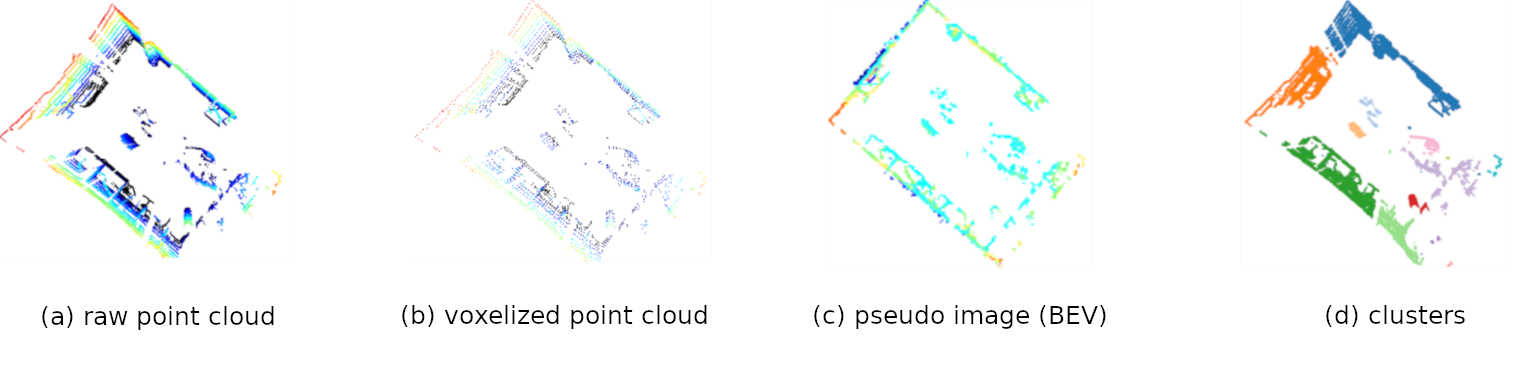
\includegraphics[width=1\textwidth]{images/Representations.png}
    \caption{Four Types of LiDAR Point Cloud Representations: 
    (a) raw point cloud, (b) voxelized (down-sampled) point cloud, (c) point cloud projected to the x-y plane, and (d) point cloud separated into clusters. In subfigure (b), each voxel is represented by its mean point. In subfigures (a) and (b), the coloring of the points relates to the height of the (mean) point. In (c), the coloring relates to the maximal height of the highest point in the pillar. In (d), the coloring encodes the cluster assignment of a point.}
    \label{fig:representations}
\end{figure}

This chapter addresses the first main contribution of this thesis by proposing a taxonomy to characterize point cloud processing pipelines.
% ToDo: number of publications
For this purpose, I surveyed more than 30 publications in the scope of point cloud segmentation and 3D object detection.
Most of these systems rely on machine learning, with deep neural networks (DNNs) becoming increasingly popular.
I identified the underlying representation of the point cloud as the major factor of variation.
It determines the required pre-processing steps and the machine learning models that we can apply.
The taxonomy distinguishes four dominant representation types.
They are illustrated in Figure \ref{fig:representations}.\\




\par Pipelines operating on the raw point cloud (a) only apply minimal pre-processing and input the points to some DNN to solve the target task. 
This approach exploits the ability of DNNs to learn an appropriate representation of the data during the training process.
\par A voxelized point cloud (b) represents the point cloud using three-dimensional pixels, also called voxels.
A voxel representation provides more structure and requires less memory than the raw point cloud.
Also, it can be processed more efficiently by leveraging 3D convolutional neural networks (CNNs).
\par Pseudo-images (c) further reduce computation and memory costs by projecting the point cloud representation to a two-dimensional image plane.
There are two dominant pseudo-image types: frontal view (FV) and bird's eye view (BEV) projections.
In both cases, the target task is typically performed by a 2D CNN.
\par Up to this point, all the pipelines rely on a DNN to perform the target task.
Although we can reduce the costs by discretizing the point cloud and projecting it to two dimensions, the representations are still quite large.
Also, deep learning models are rather complex and need many parameters.
Representing the point cloud as a set of clusters (d) is more memory efficient (\eg one feature vector per cluster), and it allows us to use less complex models, \ie support vector machines (SVMs), random
forests (RFs), or small neural networks. 
As a drawback, building this kind of representation takes more computational effort.
Also, selecting semantically meaningful features is crucial for the system's performance.\\

\par These four representation types are also found in systems that fuse point clouds with other data, \eg camera images (\ie \cite{shin2019roarnet}) or geospatial data (\ie \cite{zovathi2019}).
Some systems also fuse different representations of the same point cloud or combine them in a two-stage approach.
The underlying representations and processing techniques applied to the point cloud however are the same.
There is therefore no need to define additional classes.\\

\par The upcoming sections \ref{sec:point_based} - \ref{sec:clustering} provide more detailed insight into each class by introducing a few examples.
The final section \ref{sec:taxonomy_discuss} discusses the limitations of the taxonomy and the implications for the upcoming chapters in this thesis.

% ToDo: Figure \ref{fig:timeline} shows a timeline holding the most prominent systems over the past few years.

% \begin{figure}
%   \centering
%   

\begin{tikzpicture}[]
    \draw[snake] (0,0) -- (2,0);
    \draw[->,thick] (2,0) -- (14.5,0);(
    \foreach \x in {2,4,6,8,10,12,14}
    \draw (\x cm,3pt) -- (\x cm,-3pt);

    \draw (2,0) node[below=3pt] {2018};
    \draw (4,0) node[below=3pt] {2019};
    \draw (6,0) node[below=3pt] {2020};
    \draw (8,0) node[below=3pt] {2021};
    \draw (10,0) node[below=3pt] {2022};
    \draw (12,0) node[below=3pt] {2023};
    \draw (14,0) node[below=3pt] {2024};

    \node (2017) at (1.5, 0) {};
    \node (2016) at (1, 0) {};
    \node (2015) at (0.5,0) {};


    % --- 2015 --- %
    \node (wen) at (1.3,2)    {\textcolor{magenta}{Wen \etal (2015) \cite{wen2015}}};
    \draw[->] (0.5,1.7) -- (2015);

    % --- 2016 --- %
    \node (li) at (1, -3)    {\textcolor{blue}{Li \etal (2016) \cite{li2016}}};
    \draw[->] (li) -- (2016);

    % --- 2017 --- %
    \node (DepthCN)     at (2, 1.5)   {\textcolor{violet}{DepthCN (2017) \cite{asvadi2017}}};
    \node (MV3D)        at (1.8,1)   {\textcolor{blue}{MV3D (2017) \cite{chen2017mv3d}}};
    \draw[->] (1.5,0.7) -- (2017);
    % \node (PointNet) at (1.5, -1) {\textcolor{YellowOrange}{PointNet (2017), \cite{qi2017}}};

    % --- 2018 --- %
    % June
    \node (PIXOR)       at (2.6, -1)      {\textcolor{blue}{PIXOR \cite{yang2018pixor}}};
    % \node (PointFusion) at (3, -1.5)    {\textcolor{YellowOrange}{PointFusion\cite{xu2018pointfusion}}};
    \draw[->] (3,-0.7) -- (3,0);

    % September
    % \node (YOLO3D)      at (3.5,-2)   {\textcolor{blue}{YOLO3D \cite{ali2018yolo3d}}};
    % \draw[->] (YOLO3D) -- (3.5, 0);

    % October
    \node (AVOD)        at (3.6, -2)     {\textcolor{blue}{AVOD \cite{ku2018avod}}};
    \draw[->] (AVOD) -- (3.6, 0);

    % November
    \node (asvadi)  at (3.7, 3) {\textcolor{cyan}{Asvadi \etal \cite{asvadi2018multimodal}}};
    \draw[->] (asvadi) -- (3.7, 0);
    
    % --- 2019 --- %
    % January
    \node (zhao)    at (4.9, 1.5)   {\textcolor{magenta}{Zhao \etal \cite{zhao2019}}};
    \draw[->] (4,1.2) -- (4,0);

    % June
    \node (LaserNet)     at (5,-2.5)        {\textcolor{blue}{LaserNet \cite{meyer2019}}};
    \node (PointPillars) at (5, -3)  {\textcolor{violet}{PointPillars \cite{lang2019point-pillars}}};
    \node (RoarNet)      at (5, -3.5)    {\textcolor{YellowOrange}{RoarNet \cite{shin2019roarnet}}};
    \draw[->] (LaserNet) -- (5,0);

    % October
    \node (STD)     at (5.7,-1)     {\textcolor{YellowOrange}{STD \cite{yang2019std}}};
    \draw[->] (5.6,-0.8) -- (5.6,0);

    % November
    % \node (F-ConvNet) at (5.7, 1)   {\textcolor{YellowOrange}{F-ConvNet \cite{wang2019frustum}}};
    % \draw[->] (F-ConvNet) -- (5.7, 0);

    

    % --- 2020 --- %
    % August
    \node (3D-CVF)  at (7.4, -2)    {\textcolor{Green}{3D-CVF \cite{yoo2020-3D-cvf}}};
    \draw[->] (3D-CVF) -- (7.4,0);
    
    % September
    \node (zhang)   at (7.5, 1.5) {\textcolor{magenta}{Zhang \etal \cite{zhang2020}}};
    \draw[->] (zhang) -- (7.5,0);

    % --- 2021 --- %
    % September
    \node (BEV-Net)     at (9.5, -1)    {\textcolor{blue}{BEV-Net \cite{liu2021bev-net}}};
    \draw[->] (BEV-Net) -- (9.5,0);
    % October
    \node (RangeDet)    at (9.6, 2)     {\textcolor{blue}{RangeDet \cite{fan2021}}};
    \draw[->] (RangeDet) -- (9.6, 0);
    
    % --- 2022 --- %
    

    % --- 2023 --- %
    % May
    \node (PV-RCNN) at (12.55, 1) {\textcolor{YellowOrange}{PV-RCNN \cite{cherif2023}}};
    \draw[->] (13.35, 0.7) -- (13.35, 0);

    % September
    \node (HistoGrid)   at (13, -1)  {\textcolor{violet}{HistoGrid \cite{buerkle2023}}};
    \draw[->] (13.5, -0.7) -- (13.5, 0);

    % October
    \node (RangeFormer) at(13.6, 2) {\textcolor{blue}{RangeFormer \cite{kong2023rangeformer}}};
    \draw[->] (RangeFormer) -- (13.6, 0);
    
    %December
    \node (Zhang2023) at (14.85, 1.5) {\textcolor{YellowOrange}{Zhang \etal \cite{zhang2023}}};
    \draw[->] (13.9, 1.2) -- (13.9, 0);

    % --- 2024 --- %
    \node (ScorePillar) at (14.2,-2)    {\textcolor{YellowOrange}{ScorePillar \etal \cite{cao2024scorepillar}}};
    \draw[->] (ScorePillar) -- (14.2, 0);
    
    
    
    % Clusters
    % first paper working with LiDAR (fusion)
    % \node (szarvas) at (0,2) {\textcolor{magenta}{Szarvas \etal (2006) \cite{szarvas2006}}};
    % \draw[->] (szarvas) -- (2006);
    % first paper working solely with LiDAR (no fusion)
    % \node (kidono) at (0.5, 1.5) {\textcolor{magenta}{Kidono \etal (2011) \cite{kidono2011}}};
    % \draw[->] (kidono) -- (2011);
    % first paper in 'A-class' conference
      
    % \draw
    
    

    
    

\end{tikzpicture}
%   \caption{Landmarks of LiDAR Point Cloud Processing in the Past Decade}
%   \label{fig:timeline}
% \end{figure}


\section{Point-Based Pipelines}
\label{sec:point_based}
% general description of the pipeline
Pipelines that operate on the raw point cloud pursue an end-to-end approach.
A DNN learns how to represent the point cloud in a semantically meaningful way and how to solve the target task.
The pipeline may still pre-process the point cloud, \ie computing the Cartesian coordinates of points or limiting the field of view.
However, most publications do not explicitly discuss the input format.
We assume that most of the discussed systems rely on the Cartesian coordinates and the reflection intensity and create a three-dimensional tensor by stacking points belonging to the same frame.
This representation is, for example, proposed by Yang \etal \cite{yang2019std}.\\

\par PointNet \cite{qi2017pointnet} only relies on the Cartesian coordinates.
The points are stacked in a $n \times 3$ matrix that is then processed by a DNN including transformation, linear, activation, and pooling layers.
Figure \ref{fig:labeling_point_level} illustrates the process of point cloud segmentation. % ToDo: PointNet ++
\par PointNet and its successor PointNet++ \cite{qi2017pointnet++} have not been designed for LiDAR point clouds but serve as a backbone network in specialized systems, \ie by Shin \etal (RoarNet, \cite{shin2019roarnet}) and Zhang \etal \cite{zhang2023}.
RoarNet fuses camera and LiDAR data in a two stage approach.
It identifies object candidates in RGB images and extracts the corresponding region from the point cloud.
For each proposal, it predicts bounding box parameters and an 'objectness score'.
It thereby leverages a simplified version of PointNet as a backbone.
Zhang \etal \cite{zhang2023} combine the output representation of PointNet++ \cite{qi2017pointnet++} and two other non-LiDAR-specific DNNs with
an embedding of the distance.
These large feature vectors are then fed into an LSTM to segment the point cloud.\\

\par DNNs operating on the point-level further used in hybrid end-to-end systems to learn the representation of a voxel or pixel based on the associated points, \ie VoxelNet \cite{zhou2018voxelnet} or PointPillars \cite{lang2019point-pillars}.
These systems are however discussed in the later sections of this chapter.


\begin{figure}
    \centering
    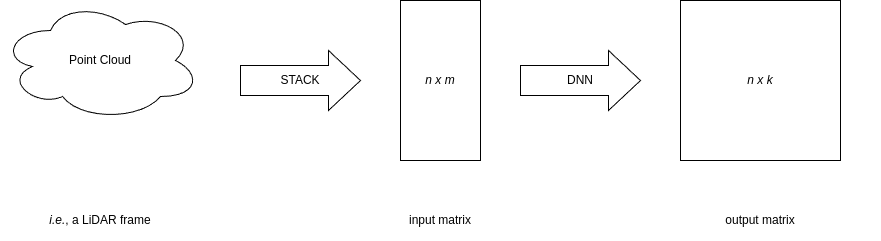
\includegraphics[width=0.9\linewidth]{images/Point_SemanticLabeling.png}
    \caption{Semantic Labeling of a Point Cloud as implemented by PointNet \cite{qi2017pointnet}: (left) A LiDAR frame consisting of $n$ points. (center) The input representation of the point cloud: each point is represented by a feature vector holding $m$ features. These vectors are stacked in a $n \times m$ matrix. (right) The DNN outputs a score for each point and each of $k$ semantic categories.
    Applying $argmax(\cdot)$ to the output extracts the index of the predicted class for each point.}
    \label{fig:labeling_point_level}
\end{figure}



\section{Voxel-Based Pipelines}
\label{sec:voxel}
Voxels are three-dimensional pixels.
We first project the point cloud to a regular 3D grid and then build the representation of each cell based on the included points.
Typically, the cells are cubic and discretize the point cloud along the x, y, and z axes, \ie \cite{zhou2018voxelnet}.
However, building the cells along spherical axes usually results in a more balanced point distribution, e.g., a lower number of empty cells.
More recent systems explore this cylindrical voxel representation, \ie \cite{zhu2021cylindrical}.\\
% \begin{figure}
%     \centering
%     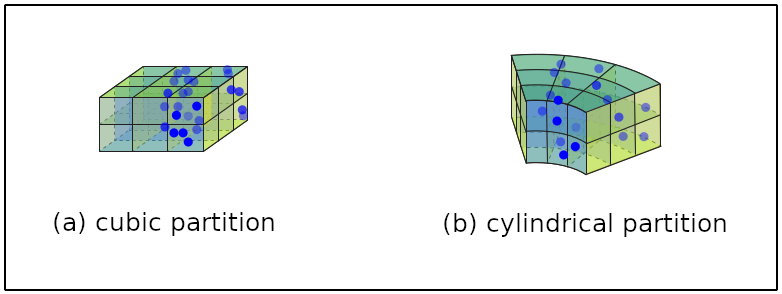
\includegraphics[width=0.75\linewidth]{images/voxelization.png}
%    \caption{Projection of a Point Cloud to a Cubic vs. a Cylindrical Grid as Illustrated by Zhu \etal \cite[p.~9940]{zhu2021cylindrical}. We can see that the cylindrical grid contains fewer empty cells.}
%    \label{fig:voxelization}
% \end{figure}

\par Early systems rely on statistical features to represent the cells. 
For example, VoxNet \cite{maturana2015voxnet} explores different ways to represent cell occupancy.
More recent systems apply an end-to-end approach. 
They learn how to represent a voxel based on the included points.
VoxelNet \cite{zhou2018voxelnet} is probably the most popular system.
Its voxel feature encoding architecture has been adopted in later systems, \ie \cite{roth2019, yang2019std}.
% ToDo: chekc 3D-CVF
3D-CVF \cite{yoo2020-3D-cvf} even uses the complete architecture of VoxelNet as a backbone.
\par Zhou \etal \cite{zhou2020e2e} pursue a different strategy.
Their system leverages learned voxel embeddings as context information.
Their detection network processes the point cloud at the point-level.
However, they enhance the input representation by annotating each point with its context.


%For that purpose, the voxelized point clouds are often represented as a 3D array with a fixed dimension of $V \times P \times F$. 
% $V$ limits the number of voxels, $P$ the number of points per voxel and $F$ refers to the number of features used to describe a point.
% $V$ is often set lower than the actual number of cells in the partition and only non-empty voxels are stacked in the array to reduce the sparsity of the array.
% The building of this representation however includes padding and sampling strategies.
% Padding is applied to fill up empty spots, \ie voxels holding less than $P$ points or point clouds with less than $V$ non-empty voxels.
% Sampling is applied to handle the overflow of voxels and point clouds.
% Zhou \etal \cite{zhou2020e2e} refer to this approach as \emph{hard voxelization}.
% The drawbacks of this strategy are obvious.
% Sampling may cause the loss of information that is relevant to the target task.
% Also, there are no guarantees regarding the sparsity of the array.
% Zhou \etal \cite{zhou2020e2e} therefore propose \emph{dynamic voxelization}.
% Each point cloud can be represented by an arbitrary number of voxels and each voxel may contain an arbitrary number of points.


% \par Further improvement has been achieved by applying dynamic voxelization \cite{zhou2020e2e}.
% Previous systems restricted the number of points per cell and applied sampling if a voxel exceeded this limit.
% Also,the number of voxels was restricted.
% This approach is referred to as hard voxelization.
% Zhou \etal \cite{zhou2020e2e} however suggest to preserve the complete mapping between points and voxels which provides a deterministic voxel embedding and more stable detection.\\



\section{Pseudo-Image Based Pipelines}
\label{sec:pseudo_image}
he key idea of a pseudo-image representation is to leverage image processing techniques to solve the target task, \eg 2D CNNs.
The first step to building the pseudo-image is to project the point cloud to an image plane.
We can find two dominating projection types: frontal view (FV) and
bird's eye view (BEV).
FV images project the points to the lateral surface of a cylinder and unroll
it.
BEV images look at the scene from above.
Figure \ref{fig:pseudo_image_projecion} illustrates these processes. 
The image plane is then discretized, computing a feature vector for each pixel.

\begin{figure}
    \centering
    \begin{subfigure}[h]{0.3\textwidth}
        \centering
         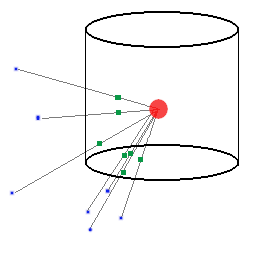
\includegraphics[width=\textwidth]{images/FV_Projection.png}
         \caption{FV Projection}
     \end{subfigure}
     \hspace{2cm}
     \begin{subfigure}[h]{0.31\textwidth}
         \centering
         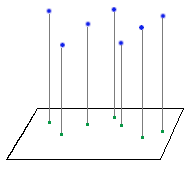
\includegraphics[width=\textwidth]{images/BEV_Projection.png}
         \caption{BEV Projection}
     \end{subfigure}
    \caption{Two Ways of Projecting a Point Cloud to a 2D Image Plane.
    The blue dots represent points in the point cloud, the green dots their projection on the image plane.
    \textbf{(a) Frontal View (FV)}: the image plane lies on the lateral surface of a cylinder that is centered at the LiDAR sensor (red dot).
    The points are moved along the directions of the corresponding laser beams.
    \textbf{(b) Bird's Eye View (BEV)}: the scene is viewed from above ($z = \infty$) and the image plane is parallel to the x-y plane.
    The points are projected downwards along the z axis.}
    \label{fig:pseudo_image_projecion}
\end{figure}

% ToDo: image representing FV vs. BEV
\newpage
\subsection{FV Images}
% projection function
FV images project the points to the image plane one by one.
To compute a point's 2D coordinates, we need to divide the azimuth and elevation by the LiDAR sensor's horizontal and vertical resolution ($\Delta_\alpha, \Delta_\omega$) respectively.:
\begin{equation}
    (x_{2D}, y_{2D}) := (\frac{\alpha}{\Delta_\alpha}, \frac{\omega}{\Delta_\omega})
    \label{eq:fv_projection}
\end{equation}
Asvadi \etal \cite{asvadi2018multimodal} further propose to increase the resolution by interpolating the values of neighbored pixels.\\

% channel information
\par An overview of the information stored in FV image feature maps is given in table \ref{tab:fv_features}.
The features mainly describe the point's location and its reflection intensity.
Meyer \etal (LaserNet) \cite{meyer2019} and Kong \etal (RangeFormer) \cite{kong2023rangeformer} further add a binary occupancy channel for each pixel.
The main difference between the surveyed systems however lies in the representation of the point location.
Asvadi \etal \cite{asvadi2018multimodal} solely use 2D depth for that purpose, which is defined as
\begin{equation}
    d_{xy} = \sqrt{x^2 + y^2}.
    \label{eq:2D depth}
\end{equation}
More recent systems rely on a larger number of features.
Kong \etal \cite{kong2023rangeformer} describe the location by the Cartesian coordinates whereas Fan \etal \cite{fan2021} use both, Cartesian and spherical coordinates.
Meyer \etal \cite{meyer2019} combine the two coordinate systems.
They report the location using the z coordinate, the radius, and the azimuth.
\par Note that Fan \etal's \cite{fan2021} FV image holds an additional channel holding the "elongation of the laser pulse beyond its nominal width" \cite[p.~2449]{sun2020WOD} which is given in the Waymo Open Dataset \cite{sun2020WOD}.
Not all LiDAR sensors however are capturing this feature.

\begin{table}
    \centering
      \begin{tabular}{c l r}
            \textbf{Property} & \textbf{Feature} & \\
            \hline
            \multirow{7}{*}{Location}
                & 2D depth (Eq. \ref{eq:2D depth}) & \cite{asvadi2017, asvadi2018multimodal}\\
                & $x$ coordinate & \cite{fan2021, kong2023rangeformer}\\
                & $y$ coordinate & \cite{fan2021, kong2023rangeformer}\\
                & $z$ coordinate & \cite{asvadi2017, chen2017mv3d, fan2021, kong2023rangeformer}\\
                & radius & \cite{chen2017mv3d, meyer2019, fan2021, kong2023rangeformer}\\
                & azimuth & \cite{meyer2019, fan2021}\\
                & elevation & \cite{fan2021}\\
            \hline
            \multirow{3}{*}{Other} 
                & reflection intensity & \cite{chen2017mv3d, asvadi2018multimodal, meyer2019, fan2021, kong2023rangeformer}\\
                & occupancy & \cite{meyer2019, kong2023rangeformer}\\
                & elongation & \cite{fan2021}\\
            \hline
            \\
    \end{tabular}
    \caption{Overview of FV Image Channel Information}
    \label{tab:fv_features}

\end{table}



\subsection{BEV Images}
% projection methodology & features
In order to create a BEV image, the point cloud is split into buckets across the x-y plane.
These are often referred to as 'pillars'.
Each bucket is then mapped to a pixel based on its position in the grid.
The pseudo image channels hold statistical information about the points included in the pillar.
Typical properties are the density or distribution of points, the height, and the reflectivity.
An overview is provided in table \ref{tab:bev_features}.
A frequent feature is some kind of normalized density which is frequently defined as 
\begin{equation}
    dens_{x,y} =\max(1.0, \frac{\log(N + 1)}{\log(64)})
    \label{eq:norm_density}
\end{equation} 
with $N$ denoting the number of points in the pillar, \ie \cite{ku2018avod}.\\% ToDo

% completion with voxel features
\par BEV images are frequently enhanced with voxel-like features.
To compute them, each pillar is split into slices of equal height along the z axis.
Such features often represent the distribution of points in the pillar.
In example, PIXOR's \cite{yang2018pixor} BEV image holds an occupancy bit for each slice.
Similarly, Ku \etal \cite{ku2018avod} propose to compute the maximal height per slice.
% (a) PIXOR
\par PIXOR \cite{yang2018pixor} in example computes the mean reflectivity across the pillar.
It further slices each pillar along the z axis and records an occupancy bit for each voxel.
Similarly, AVOD \cite{ku2018avod} computes the maximal height for each slice. 
\par Liu \& Niu \cite{liu2021bev-net} however compared the performance of their system when using PIXOR's \cite{yang2018pixor} BEV image representation to a three channel BEV image holding the mean reflection intensity, the maximal height, ad the normalized density.
Their results imply that the smaller representation decreases the time to process the point cloud and may still result in more accurate classification and bounding box predictions.\\

% learned BEV representation
\par Just as for the voxels, there are end-to-end systems that learn the representation of each pillar based on the included points.
Probably the most popular example of such systems is PointPillars \cite{lang2019point-pillars}.
It has been very successful and is applied to detect object proposals in more sophisticated systems, \ie \cite{zovathi2019, kloeker2020}.
The approach has lately been adopted by ScorePillar \cite{cao2024scorepillar}.\\

\begin{table}[]
    \centering
    \begin{tabular}{c l r}
            \textbf{Property} & \textbf{Feature} & \\
            \hline
            \multirow{2}{*}{Height}
                & maximal height & \cite{beltran2018birdnet, simon2018complex-yolo, liu2021bev-net}\\
                & slice-wise maximal height\footnote{Note that this is a voxel-like feature} & \cite{chen2017mv3d, ku2018avod}\\
            \hline
            \multirow{2}{*}{Density \& Distribution} 
                & normalized density (see Eq. \ref{eq:norm_density}) & \cite{chen2017mv3d, beltran2018birdnet, ku2018avod, simon2018complex-yolo, liu2021bev-net}\\
                & slice-wise occupancy bits & \cite{yang2018pixor, luo2018FaF, liu2021bev-net}\\
            \hline
            \multirow{2}{*}{Reflection Intensity} 
                & mean reflection intensity& \cite{beltran2018birdnet, yang2018pixor, liu2021bev-net}\\
                & $I$ of the highest point & \cite{chen2017mv3d, simon2018complex-yolo}\\
            \hline
            \\
    \end{tabular}
    \caption{Overview of BEV Image Channel Information}
    \label{tab:bev_features}
\end{table}


\section{Clustering Based Pipelines}
\label{sec:clustering}
% general description of the pipeline and it's building blocks
Pipelines making use of clustering typically follow a two stage approach, first identifying a set of candidate objects (represented by the clusters) which are then verified (\eg classified).
At the pre-processing stage, background or ground points are removed.
Some systems may apply further pre-processing, \ie region of interest extraction or denoising.
The remaining points are then clustered following either a density-based (\eg some variation of DBSCAN \cite{ester1996}, see \cite{gao2023, zhao2019}) or distance-based approach (\ie \cite{wen2015, zhang2020}).
\par In a next step, the cluster is then represented by a feature vector which often holds statistical information about the included points.
Other features describe the cluster's shape and location.
An overview of cluster features is provided in table \ref{tab:cluster_features}.
\par For classification, clustering based systems leverage less complex machine learning models, \ie support vector machines (SVMs, see \cite{lin2018, zhang2020} or small neural networks (see \cite{zhao2019}). 
Wen \etal \cite{wen2015} even perform the object verification using a single decision criterion on the eigenvalues of the cluster's 3D covariance matrix.\\

\begin{table}
    \centering
    \begin{tabular}{c l r}
        \textbf{Property} & \textbf{Feature} & \\
        \hline
        \multirow{7}{*}{Point Distribution} 
            & 2D/3D covariance matrix & \cite{kidono2011, wen2015}\\
            & normalized moment of inertia & \cite{kidono2011}\\
            & 'slice feature' & \cite{kidono2011}\\
            & point distribution histograms & \cite{zhang2020, kidono2011}\\
            & number of points & \cite{lin2018, zhao2019}\\
            & standard deviation of locality & \cite{zhang2020}\\
            & direction of distribution & \cite{zhao2019}\\
        \hline
        \multirow{6}{*}{Shape} 
            & volume & \cite{lin2018}\\
            & ratio $\frac{H}{L}$ & \cite{lin2018}\\
            & ratio $\frac{H}{W}$ & \cite{lin2018}\\
            & base area & \cite{zhang2020}\\
            & dimensions $L, W, H$ & \cite{zhang2020}\\
        \hline
        \multirow{3}{*}{Location} 
            & distance & \cite{lin2018, kidono2011, zhao2019}\\
            & mean point & \cite{zhao2019, zhang2020}\\
            & bounding box & \cite{zhao2019}\\
        \hline
        \multirow{3}{*}{Reflectivity}
            & distribution histogram & \cite{kidono2011}\\
            & mean & \cite{lin2018, kidono2011}\\
            & standard deviation & \cite{lin2018, kidono2011}\\
         \hline
        Movement & velocity & \cite{lin2018}\\
        \hline
         \\
    \end{tabular}
    \caption{Cluster Representation Features for Classification}
    \label{tab:cluster_features}
\end{table}

% 'prominent examples' -> ToDo?

% applications in hybrid or fusion approaches
\par Clustering is also a common primitive in pipelines that fuse LiDAR point clouds with some other data stream.
The clusters serve as object candidates and are projected to the other data stream for verification.
In example, Wen \etal \cite{wen2015} identify traffic signs in a point cloud and project the corresponding points to a camera image of the same scene.
The image is then used to identify the sign type.\\


\section{Intermediary Discussion}
\label{sec:taxonomy_discuss}
This chapter introduced a taxonomy for point cloud processing pipelines based on the input representation of the point cloud to the machine learning model that performs the target taks.
It identifies four major classes: raw point clouds, voxelized point clouds, pseudo images, and clusters.
For pseudo images, we can further distinguish two subtypes: frontal view and bird's eye view images.
Note that this taxonomy is not all-encompassing as there are other representations such as frustums (\ie \cite{wang2019frustum}), graphs (\ie \cite{}) or line segments (\ie \cite{}).
The taxonomy however describes the most common representation formats.\\

\par From a processing point of view, the four classes are distinguished by two processing techniques: (1) point grouping and (2) projection to two dimensions.
Raw point clouds and FV images both represent each point individually. FV images however map the point cloud to an image plane.
Similarly, a BEV image can be described as a voxelized point cloud projected to the x-y plane.
Both representation aggregate information from several points.
Clusters do so as well.
In order to extract clusters from a point cloud, one however needs to apply a different aggregation approach.
While the point cloud is split 'top-down' in order to create voxels or pillars, the clustering techniques used to cluster the point clouds all work 'bottom-up', starting from individual points and grouping them if some criterion is met.
\par This perspective on the point cloud taxonomy is visualized in figure \ref{fig:processing_representation} and it is the starting point of the further contents of this thesis.
In the next chapter, I will further break up the processing steps required to build the different point cloud representations and formalize them in a point cloud data model.

\begin{figure}
    \centering
    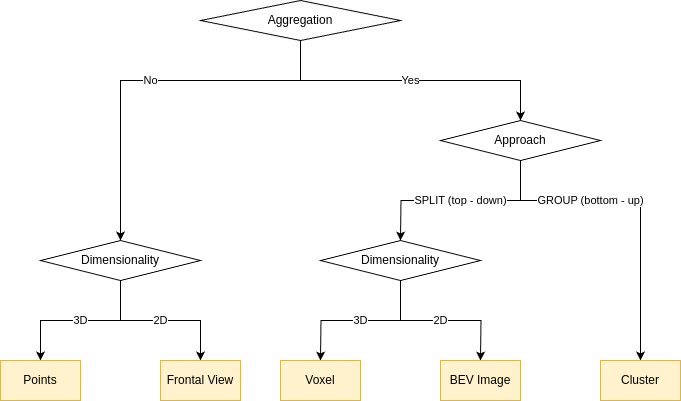
\includegraphics[width=0.8\linewidth]{images/taxonomy_hierarchy.png}
    \caption{Point Cloud Representations from a Processing Point of View}
    \label{fig:processing_representation}
\end{figure}



% \section{Other Approaches}
% \label{sec:pipeline_other}
% frustum sequence + learned
% \par Another pattern is to use an existing DNN in data fusion.
% In example, F-ConvNet \cite{wang2019frustum} aims at verifying object proposals that were previously identified from an RGB imge.
% For each proposal, the system extracts a sequence of frustums.
% The points contained in a frustum are then input into PointNet \cite{qi2017pointnet} in order to learn a representation vector.
% All vectors belonging to the same object proposal are then stacked and passed through a CNN which performs both, classification and 3D bounding box prediction.\\


% ToDo: Graphs
% \par Another set of systems builds a graph representation of the point cloud.\\

% Energy Minimization
% \par A quite unique approach is proposed by Xiao \etal \cite{xiao2016}.
% They aim for simultaneous detection and tracking of pedestrians.
% This is achieved by removing the background from the point cloud projecting the remaining points into a $(x, y, t)$ space which is then split along the time axis into frames.
% Xiao \etal then formulate the detection-and-tracking task as an energy minimization problem.
% For each set of consecutive frames, they extract trajectory segments (tracklets) and associate all points with the tacklet that are 'close enough' to the line segment.
% Finally, they associate tracklets form consecutive frame transitions with each other.
% Points and tracklets are only connected if they reduce the value of the global energy function.



\chapter{Point Cloud Data Model}
\label{cha:dataModel}
This chapter sketches a data model that formalizes LiDAR generated point clouds and the corresponding processing techniques.
The first section \ref{sec:domain} defines the underlying domain and section \ref{sec:ops} introduces basic building blocks.
In the last section \ref{sec:model_examples}, I will illustrate how to generate some of the previously discussed representations using the model's building blocks.

\section{Domains}
\label{sec:domain}
Data points collected by a LiDAR sensor typically hold the coordinates of the point of reflection, either in spherical or Cartesian coordinates, and the intensity of the reflected laser beam.
All of these features are numerical.
We therefore define the feature space as 

\begin{equation*}
    \mathcal{F} := \mathbb{R}.
\end{equation*}

Each point can now be described by an arbitrary number of features that can be stacked in a feature vector.
The point domain is formalized as
\begin{equation*}
    \mathcal{P} := \mathcal{F}^*.
\end{equation*}

A point cloud consists of an arbitrary number of points.
We can describe it as a vector of points or a matrix of features.
The point cloud domain is therefore defined as
\begin{equation*}
    \mathcal{C} := \mathcal{P}^*.
\end{equation*}
Note that in order to form a point cloud from a set of points, all points must hold the same set of features in the same order as the semantics of a feature is implied by its absolute position.
Also, the points could be organized in columns or rows.
For this thesis, each point is represented by a row.
$c \in \mathcal{F}^{nxm}$ therefore describes a point cloud holding $n$ points, each being described by $m$ features.

\section{Operations}
\label{sec:ops}
\subsection{Filtering}
The filtering operation maps one point cloud to another, removing some points based on a criterion.
A filter $f$ can therefore be defined as
\begin{align*}
    f : \hspace{2mm} & \mathcal{C} \rightarrow \mathcal{C}\\
                    & c \mapsto c'   
\end{align*}
Note that if $c \in \mathcal{F}^{m \times n}$, then $c' \in \mathcal{F}^{m \times k}$ and $k \leq n$.
Also, a filter can only remove points from a cloud.
If we define the columns of the feature matrices as set, we can express this requirement as $c' \subseteq c$.


\subsection{Grouping}
Grouping refers to operations that extract one or several point clouds from an input point cloud.
\begin{align*}
    g : \hspace{2mm} & \mathcal{C} \rightarrow \mathcal{C}^*\\
                    & c \mapsto {c'_1, c'_2, ... c'_k}.   
\end{align*}
In general, each of the outputs $c'_i$ is a strict subset of $c$.
We may further require the output point clouds to be pairwise disjoint.\\

\par There are two strategies when it comes to grouping points: top-down or bottom-up.
Top-down strategies start from the whole point cloud and subsequently divide it into subsets.
This approach is followed in discretization, \eg to build a voxel or BEV image representation of the point cloud.
Bottom-up strategies start from individual points and subsequently group them.
This approach is typically pursued in clustering.\\

\par Another perspective on grouping is to see it as an annotation of each point with one or several features that describe their set memberships.
As an example, in order to map a point to a voxel, we can assign an index for each of the three dimensions, \ie $x$, $y$, and $z$.
Each point is hence annotated with a tuple $(i_x, i_y, i_z)$.
Similarly, we may express the membership to some pillar by two indices, or use a cluster-id to assign points to clusters.



\subsection{Arithmetical and Analytical Operations}
An arithmetical operation, \eg addition, subtraction, multiplication, or division, takes two features as an input and outputs a single feature:
\begin{align*}
    arith: \hspace{2mm} & \mathcal{F} \times \mathcal{F} \rightarrow \mathcal{F}\\
                    & (f_1, f_2) \mapsto f'.
\end{align*}
In most of the cases observed in out survey, the input features are either taken from the same feature vector (\ie point) or one feature is taken from the feature vector and the other one is constant.
As an example for the first case, let's have a look at the computation of the 2D-depth of a point.
For each point with x and y coordinates $(x, y)$, we need to evaluate
\begin{align*}
    d = \sqrt{x^2 + y^2}
\end{align*} 
of a point is an example for the first case.
In a first step, we square the x value and the y value.
The results are then added.
Finally, we need to draw the square root - this is however not an arithmetical operation.
\par As an example for the second case, we compute the index $i_x$ in the process of point cloud voxelization.
As the field of view of the LiDAR sensor limited, the x coordinate is bounded by some values $[X_{MIN}, X_{MAX}]$.
We further aim at dividing the point cloud into equally thick slices of width $\Delta_X$ along the x axis.
For each point with x coordinate $x$, we now need to evaluate
\begin{align*}
    i_x \hspace{2mm} = \lfloor\frac{x - X_{MIN}}{\Delta_X}\rfloor.
\end{align*}
% ToDo ...
\\

\par Analytical functions can take an arbitrary number of features as input, provided that the vector lies in the function's definition range.
In our survey, we only observed a small number of functions, namely the trigonometric functions $\sin{}, \arcsin{}, \cos{}$, and $\arctan{}$, logarithm functions $\log$, and the square root function $\sqrt{\cdot}$.
Except for $\arctan2$, all of them are defined on $\mathbb{R}$ or some subspace of it.
For our purpose, we will therefore define an analytical function $A$ as:
\begin{align*}
    A: \hspace{2mm} & \mathcal{F} \rightarrow \mathcal{F}\\
                    & f \mapsto f'
\end{align*}



\subsection{Aggregation}
Feature aggregation is performed to represent a group of points in a BEV image, by a single Feature vector, \eg a cluster, a voxel or a pillar in a BEV image.
This vector typically contains statistical information about the aggregated points.
Each position in this vector is computed by an aggregation operation:
\begin{align*}
    agg: \hspace{2mm} & \mathcal{C} \rightarrow \mathcal{F}\\
                      & c \mapsto f
\end{align*}
We may therefore need to apply several aggregation operations to the same point set in parallel.\\
\par
As for analytical functions, we can only observe a small set of distinct aggregation operations, namely counting the number of points in a set, and computing the maximum, minimum, mean, variance, or standard deviation of some feature. 
More complex features representing the point set can be computed by applying arithmetical and analytical operations to the aggregated feature vector.

\section{Intermediary Discussion}
This chapter aimed at defining a data model to formalize LiDAR generated point clouds and processing techniques that are applied to them.
For the limited scope of this thesis, the set of operations is small.
On the point/vector level, we may want to remove points or feature vectors from a point cloud representation (\emph{filtering}) or annotate them with one or several features to indicate their set memberships (\emph{grouping}).
On the feature level, we may want to \emph{aggregate} features across such set or compute new features by applying \emph{arithmetical and analytical operations}.
These feature-level operations are summarized in table \ref{tab:agg_ops}.\\
\par We further showed that in the process of point cloud discretization, \eg voxelization or pillarization, the indices defining a set membership can be obtained by applying arithmetical operations.

\begin{table}[]
    \centering
    \begin{tabular}{c|c|l|c}
        \hline
        \multirow{5}{*}{\rotatebox[origin=c]{90}{Analytical}} 
            & \multirow{5}{*}{$\mathcal{F} \rightarrow \mathcal{F}$}
                & sine & $\sin{(\cdot)}$\\
                & & arcsine & $\arcsin{(\cdot)}$\\
                & & cosine & $\cos{(\cdot)}$\\
                & & logarithm & $\log{(\cdot)}$\\
                & & square root & $\sqrt{\cdot}$\\
        \hline
        \multirow{5}{*}{\rotatebox[origin=c]{90}{Arithmetical}} 
            & \multirow{4}{*}{$\mathcal{F}^2 \rightarrow \mathcal{F}$}
                & addition & $+$\\
                & & subtraction & $-$\\
                & & multiplication & $\cdot$\\
                & & division & $\div$\\
                &&\\
        \hline
        \multirow{5}{*}{\rotatebox[origin=c]{90}{Aggregation}} 
            & \multirow{5}{*}{$\mathcal{F}^* \rightarrow \mathcal{F}$}
                & counting & $count(*)$ \\
                & & minimal value & $min(\cdot)$\\
                & & maximal value & $max(\cdot)$\\
                & & mean value & $mean(\cdot)$\\
                & & variance of a value & $var(\cdot)$\\
         \hline
    \end{tabular}
    \caption{Overview of Feature-Level Operations Supported in the Point Cloud Data Model}
    \label{tab:agg_ops}
\end{table}




\chapter{LiDAR Processing Unit (LPU)}
\label{cha:LPU}
This chapter proposes a hardware architecture for processing LiDAR point clouds. 
A core of such an architecture will be termed a LiDAR Processing Unit (LPU).
An LPU comprises several building blocks, namely filter units (section \ref{sec:filter}), arithmetic units (\ref{sec:ArU}), and aggregation units (\ref{sec:AgU}).
Figure \ref{fig:unit} depicts the interfaces of such a subunit.
It processes a single feature vector (\eg a point) at a time, thereby passing it from left to right.
The corresponding interfaces are equal for all building blocks.
We can therefore stack them in an arbitrary order.
The bottom input (configuration) allows to program the unit.
Its format and content depend on the unit type.
Table \ref{tab:unit_config} provides an overview.\\
\par The first three sections of this chapter describe the building blocks of the LPU and their configuration.
Sections \ref{sec:LPU_architecture} and \ref{sec:LPU_instructions} then explain how to construct an LPU from the subunits and how to program it.
\begin{figure}
    \centering
    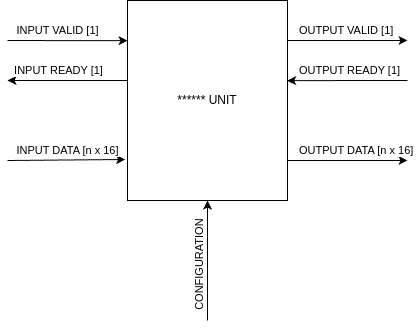
\includegraphics[width=0.4\linewidth]{images/Unit_General.png}
    \caption{General Architecture of an LPU Sub-Unit. 
    The numbers in brackets define the port sizes where $n$ denotes the number of features in a vector.}
    \label{fig:unit}
\end{figure}


\section{Filter Unit}
\label{sec:filter}
A filter unit removes feature vectors from the data stream based on one or several criteria given in its configuration.
Each criterion is evaluated by a filter cell.
It takes a single feature $f$ as input.
Its configuration consists of a value $REG$ stored in some register, and a four-bit opcode that defines a comparison operator $\circ$.
The cell outputs one if and only if the expression $f \circ REG$ is true.
Table \ref{tab:filter_cell_opc} defines the cell-level opcodes.
Note that the most significant bit indicates whether the values $f$ and $REG$ are signed and therefore does not matter for the definition of $\circ$.\\

\par The unit wraps the cells.
It selects the input feature to each cell based on a feature index passed in the configuration.
It further aggregates the cell outputs into a global result based on a unit-level opcode, see Table \ref{tab:filter_unit_opc}.
Note that only active cells should be considered in the evaluation.
For that purpose, the configuration further contains a bit vector to indicate the activation state for each cell.
A feature vector is only forwarded, if the aggregation outputs one.

\begin{table}[]
    \begin{subtable}[h]{0.5\textwidth}
        \centering
        \begin{tabular}{c|c}
            \textbf{Opcode} & \textbf{Criterion} \\
            \hline
            *000 & $f < REG$\\
            *001 & $f == REG$\\
            *010 & $f > REG$\\
            *100 & $f \geq REG$\\
            *101 & $f \neq REG$\\
            *110 & $f \leq REG$\\
           \hline
        \end{tabular}
        \caption{Cell-Level}
        \label{tab:filter_cell_opc}
    \end{subtable}
    \begin{subtable}[h]{0.5\textwidth}
        \centering
        \begin{tabular}{c|c}
            \textbf{Opcode} & \textbf{Operation} \\
            \hline
            00 & $OR$\\
            01 & $AND$\\
            10 & $NOR$\\
            11 & $NAND$\\
            \hline
        \end{tabular}
        \caption{Unit-Level}
        \label{tab:filter_unit_opc}
    \end{subtable}
    \caption{Filter Unit Opcodes. 
        Cell-level opcodes (a) describe the comparison operation for a single criterion. 
        Unit-level opcodes (b) define th}
\end{table}


\section{Arithmetic Unit}
\label{sec:ArU}
Arithmetic units implement arithmetical and analytical functions.
As filter units, they are subdivided into cells that each perform a single  operation.
They take two features and output the result as a single feature.
The operation is again configured by some opcode. % ToDo: size of opcode?
The opcode indicates (1) whether the feature values are signed, (2) whether the operation is binary (arithmetical) or unary (analytical) and (3) what operation to perform in that group.\\

\par On the unit level, we select the cells' input features. These are either two features from the input feature vector (specified by some input feature indices) or one feature and a constant value that is stored in some register.
For each cell, there is a bit indicating whether to use the register or not.
\par On the unit level, we can also select what features to output.
For that purpose, we can pass $n$ output feature indices, where the range $[0, n-1]$ is used to select input features and $[n, n+c-1]$ for the computed features that are output by the cells.\\



\section{Aggregation Unit}
\label{sec:AgU}

\begin{table}
    \centering
    \begin{tabular}{c|l|r}
        \textbf{Type} & \textbf{Purpose} & \textbf{\# bits}\\
        \hline
        \multirow{5}{*}{Filter Unit}
            & unit opcode & $2$ \\
            & cell activation & $c$ \\
            & cell feature indices & $c \times \lfloor \log_2(n) + 1 \rfloor$ \\
            & cell opcodes & $c \times 4$\\
            & cell registers & $c \times 16$\\
        \hline
        \multirow{5}{*}{Arithmetic Unit}
            & use\_register & $c$ \\
            & cell feature indices & $c \times \lfloor \log_2(n) + 1 \rfloor$\\
            & cell registers & $c \times 16$ \\
            & cell opcodes & $c \times 3$\\
            & output feature indices & $n \times \lfloor \log_2(n + c) + 1 \rfloor$\\
        \hline
        \multirow{2}{*}{Aggregation Unit}
            & cell feature indices & $c \times \lfloor \log_2(n) + 1 \rfloor$\\
            & cell opcodes & $c \times 3$\\
        \hline
    \end{tabular}
    \caption{Unit Configuration Parameters and Their Sizes. 
    $n$ denotes the number of features per vector, $c$ the number of cells in a subunit.}
    \label{tab:unit_config}
\end{table}



\section{LPU Architecture}
\label{sec:LPU_architecture}

\section{Instruction Set \& LPU Programming}
\label{sec:LPU_instructions}

\chapter{Experiments}
\label{cha:Experiments}
%\chapter {The Validation}
%In which you show how well the solution works.

\chapter{Discussion}
\label{cha:discuss}
%In which we step back, have a critical look at the entire work, then conclude, and learn what lies beyond this thesis.

% ToDo: Limitations and Future Work


%END Doc
%-------------------------------------------------------
\bibliography{references}
\bibliographystyle{plain}

\chapter*{\centering Appendix}
\section*{System Classification}
% \begin{tabular}{l|l l l}
%     & \textbf{Pure} & \textbf{Fusion} & \textbf{Hybrid} \\
%     \hline
%     \multirow{5}{*}{Point Based}
%        &
%            & RoarNet (2019, \cite{shin2019}) 
%            &  \textbf{PointPillars (2019, \cite{lang2019point-pillars})} \\
%        & \textbf{STD \cite{yang2019std}}& & ScorePillar (2024, \cite{cao2024}) \\
%        & \textbf{PV-RCNN (2023, \cite{cherif2023})} & &\\
%        & \textbf{Zhang \etal (2023, \cite{zhang2023})}& &\\
%        & Wu \etal (2024, \cite{})& & \\
%     \hline
%     \multirow{5}{*}{Voxel Based}
%        & 
%            & 
%            & \\
%        & 
%            & 
%            & \\
%        & 
%            & 
%            & \\
%        & 
%            & 
%            & \\
%        & 
%            & 
%            & \\
%     \hline
%     \multirow{5}{*}{Pseudo Image Based}
%        & BirdNet (2018, \cite{beltran2018birdnet}) 
%            &  \textbf{MV3D (2017, \cite{chen2017mv3d})}
%            & \textbf{PointPillars (2019, \cite{lang2019point-pillars})}\\
%        &  \textbf{PIXOR (2018, \cite{yang2018pixor})} 
%            &  \textbf{Asvadi \etal (2018, \cite{asvadi2018multimodal})}
%            & HistoGrid (2023, \cite{buerkle2023})\\
%        & \textbf{YOLO3D (2018, \cite{ali2018yolo3d})} 
%            & \textbf{AVOD (2018, \cite{ku2018avod}}
%            & \\
%        & \textbf{LaserNet (2019, \cite{meyer2019})} 
%            & \textbf{Point-DETR3D 2024, \cite{gao2024})} 
%            & \\
%        & \textbf{RangeDet (2021, \cite{fan2021})}
%            & 
%            & \\
%     \hline
%     \multirow{5}{*}{Clustering Based}
%        & Kidono \etal (2011, \cite{kidono2011})
%            & Szarvas \etal (2006, \cite{szarvas2006})
%            & HistoGrid (2023, \cite{buerkle2023})\\
%        & Lin \etal (2018, \cite{lin2018}) 
%            & Wen \etal (2015, \cite{wen2015}) 
%            & \\
%        & \textbf{Zhao \etal (2019, \cite{zhao2019})}
%            & 
%            &\\
%        & \textbf{Zhang \etal (2020, \cite{zhang2020})} 
%            & 
%            & \\
%        & & & \\
%     \hline
%     % \multirow{5}{*}{Others} & Premebida \etal (2009, \cite{premebida2009})  & Zhang \etal (2014, \cite{zhang2014}) & \\
     %   & Xiao \etal (2016, \cite{xiao2016}) & & \\
     %   & VoxelNet (2018, \cite{zhou2018}) & & \\
     %   & & & \\
     %   & & & \\
     % \hline
% \end{tabular}

\end{document}
